\chapter{Manifolds}

Roughly speaking, a ``manifold'' is a locally flat geometric object without pre-ordained local coordinate systems. Before we formalize what we mean by this, it's useful to philosphize a bit. First of all, let's think about what ``locally flat'' means. Consider, for example, the surface of the earth. On the one hand, we know that it's a sphere (approximately, at least). On the other hand, we also know from personal experience that the curvature of the earth is irrelevant in situationsn where everything of concern is within a few miles of us. The earth looks flat. It is in this sense that the surface of the earth is ``locally flat.'' 

When we have such a locally flat geometric object, it's often useful to introduce ``local coordinate systems.'' For example, we talk about things being ``in front of'' us or being ``behind'' us in our everyday lives, despite the fact that, if you go far enough forward, you'll eventually end up behind where you started! In other words, ``in front of'' and ``behind'' make no sense if we're thinking globally (ie, if we're thinking at the level of the entirety of the earth). They only make sense ``locally,'' but despite that, they're incredibly useful notions in everyday life. Similar considerations apply with ``left'' and ``right.''

It's also useful to allow local coordinate systems to change depending on the situation we're in. Returning to the example of ``in front of'' and ``behind,'' notice that these notions don't refer to absolute directions: if you turn 90$^\circ$ in some direction, what was ``in front of'' you before you turned isn't ``in front of'' you anymore. After your $90^\circ$ turn, there's now a new useful notion of ``in front of.'' In other words, changing the situation you're in has made a different local coordinate system useful.

Let's now return to the sentence we started with, that ``manifolds are locally flat geometric objects without pre-ordained local coordinate systems.'' We'll see below how to formalize ``locally flat'' mathematically. The way we'll avoid having pre-ordained local coordinate systems is by remembering \emph{all possible choices} of local coordinate systems! 

It's also worth remarking that this chapter marks a somewhat significant turning point in our meditation of derivatives and tangents. We began \cref{single} with the observation that we could formalize our intuitive idea of ``tangent line'' using  derivatives. In the next chapter, we'll see that, in the abstract setting of manifolds, we can formalize the idea of ``tangent vector,'' and then use it to define an even further generalization of the derivative. 

\section{Definition of a manifold}

At this point, we will need to use the language of topological spaces. If you've seen metric spaces but not topological spaces, you should skim through \cref{topological-spaces-basics} (in particular, at least \cref{topological-space-definition,metric-to-topological,continuous-definition,open-map-definition,homeomorphism-definition}).

\subsection{Charts}

Throughout this section, let $X$ be a topological space.\index{topological space} Recall that we want for $X$ to be ``locally flat.'' Formally, this means that we can cover $X$ with open subsets, each of which is ``flat'' in the sense that it is homeomorphic to an open subset of $\R^n$. Notice that, if we remember not just the fact that each open subset $U$ in that cover is homeomorph\emph{ic} to $\R^n$, but the actual homeomorph\emph{ism}, then we can transfer the usual coordinate system on $\R^n$ through the homeomorphism onto $U$. In other words, a homeomorphism between $U$ and an open subset of $\R^n$ tells us both that $U$ is ``flat,'' and gives us a coordinate system on $U$. This is precisely what's accomplished by the following definition. 

\begin{definition}[Chart] \index{chart}
	A \emph{chart} on $X$ is a pair $(U, x)$ consisting of an open subset $U \subseteq X$ and a continuous, open\index{open!open map}, and injective function $x : U \to \R^n$ for some $n$. 
	\begin{itemize}
		\item The integer $n$ is called the \emph{dimension} of the chart, and write $\dim (U,x)$ to denote it. 
		\item The function $x$ is called the \emph{coordinate function} of the chart. 
		\item If $p \in X$, we say that the chart $(U,x)$ \emph{contains} $p$ if $p \in U$. 
		\item For all $i = 1, \dotsc, n$, we let $x_i := \pi_i \circ x$. For any $p \in U$, the real numbers $x_1(p), \dotsc, x_n(p)$ are called the \emph{coordinates of $p$ with respect to $(U,x)$}.\index{coordinates}
	\end{itemize} 
\end{definition}

\begin{remark} \label{recentering-chart}
	If $(U,x)$ is a chart on $X$ and $p \in U$  is a point, we can ``recenter the chart at $p$'' by replacing $x$ with the function $x' = x - x(p)$. In other words, if $x' = x - x(p)$, then $(U, x')$ is also a chart, and we have $x'(p) = 0$.
\end{remark}

\begin{exercise} \label{polar-representation}
	Let $X = \R^2$ and let $U$ denote $\R^2$ minus the non-negative real axis. Let $\text{polar} : U \to \R^2$ be the function which sends a point $p$ to its polar representation $(r(p), \theta(p))$, where $r(p) = |p|$ and $\theta(p)$ is the angle in radians strictly between 0 and $2\pi$ formed between $P$ and the non-negative real axis. Show that $(U, \text{polar})$ is a chart. Calculate the coordinates of $(1,1) \in \R^2$ with respect to $(U, \text{polar})$. 
\end{exercise}

\subsection{Compatibility of charts}

Charts formalize the idea of local coordinate systems; the following formalizes the idea of \emph{changing} local coordinate systems. 

\begin{definition}[Transition function] \label{transition-map} \index{transition function}
	Suppose $(U, x)$ and $(U', x')$ are charts on $X$. The \emph{transition function} from $(U, x)$ to $(U', x')$ is the function $x' \circ x^{-1}$. 
	\[ \begin{tikzcd}
	x(U \cap U') \ar{r}{x^{-1}} & U \cap U' \ar{r}{x'} & x'(U \cap U')
	\end{tikzcd} \]
\end{definition}

\begin{definition}[Compatibility of charts] \index{compatibile} \label{compatibility}
	The two charts $(U, x)$ and $(U', x')$ on $X$ are \emph{smoothly compatible}, or just \emph{compatible}, if both of the transition maps between $(U, x)$ and $(U', x')$ are smooth. 
\end{definition}

\begin{exercise} \label{polar-compatible-with-identity}
	Let $\id : \R^2 \to \R^2$ denote the identity map and $\text{polar} : U \to \R^2$ the polar representation map from \cref{polar-representation}. Show that $(\R^2, \id)$ and $(U, \text{polar})$ are compatible charts. 
\end{exercise}

\begin{exercise}
	Suppose $(U, x)$ is a chart and $p \in X$ is a point. Consider the recentered chart $(U, x')$ where $x' = x - x(p)$, as in \cref{recentering-chart}. Show that $(U, x)$ and $(U, x')$ are compatible. 
\end{exercise}

\begin{exercise} \label{compatibility-not-equivalence-relation}
	Show that the relation ``is compatible with'' is \emph{not} an equivalence relation on the set of all charts. 
	\begin{hint}
		The function $x \mapsto x^3$ is a smooth homeomorphism $\R \to \R$, but its inverse is not differentiable. 
	\end{hint}
\end{exercise}

\begin{exercise} \label{dimension-well-defined}
	Suppose $(U, x)$ and $(U', x')$ are compatible charts and that the intersection $U \cap U'$ is nonempty. Show that $\dim(U,x) = \dim(U',x')$. 
	\begin{hint}
		Pick a point $p \in U \cap V$, and consider the derivatives of $x' \circ x^{-1}$ at $x(p)$ and of $x \circ x'^{-1}$ at $x'(p)$. 
	\end{hint}
\end{exercise}

\subsection{Atlases and manifolds}

\begin{definition}[Atlas] \index{atlas} \index{atlas!maximal atlas} \index{maximal atlas|see {atlas, maximal atlas}}
	An \emph{atlas} on $X$ is a collection $\mathscr{A}$ of compatible charts such that covers $X$. In other words, a collection $\mathscr{A}$ of charts is an atlas if every pair of charts is compatible, and \[ \bigcup_{(U, x) \in \mathscr{A}} U = X. \]
	If $\mathscr{A}'$ is also an atlas and $\mathscr{A}' \subseteq \mathscr{A}$, we say that $\mathscr{A}'$ is a \emph{sub-atlas} of $\mathscr{A}$. An atlas is \emph{maximal} if there is no strictly larger atlas containing it.
\end{definition}

\begin{exercise}[Existence and uniqueness of maximal atlases] \label{existence-maximal-atlas}
	Prove that every atlas $\mathscr{A}$ is contained in a unique maximal atlas.\index{atlas!maximal atlas} 
	\begin{hint}
		Let $\mathscr{A}'$ be the set of all charts that are compatible with all of the charts in $\mathscr{A}$. Prove that $\mathscr{A}'$ is an atlas (caution: keep \cref{compatibility-not-equivalence-relation} in mind). Then prove that it is maximal, and that it is the only maximal atlas containing $\mathscr{A}$. 
	\end{hint}
\end{exercise}

This leads us to the following definition.

\begin{definition}[Manifold] \index{manifold} \index{smooth manifold|see {manifold}}
	A \emph{smooth manifold}, or just a \emph{manifold}, is a pair $(X, \mathscr{A}_X)$ where $X$ is a topological space and $\mathscr{A}_X$ is a maximal atlas. Often, we just write ``$X$'' in place of the pair $(X, \mathscr{A}_X)$. Sometimes the maximal atlas $\mathscr{A}_X$ is called the \emph{manifold structure} or the \emph{smooth structure} on $X$.
\end{definition}

\Cref{existence-maximal-atlas} tells us that any not-necessarily-maximal atlas on a topological space $X$ can be extended uniquely to a maximal atlas, thus giving $X$ the structure of a manifold. When constructing examples, we will usually give an explicit non-maximal atlas and then use \cref{existence-maximal-atlas} to extend it to a maximal atlas; it is difficult to describe maximal atlases explicitly. But it is often convenient for theorem statements and abstract proofs to assume that the atlas that the manifold comes equipped with is already maximal, which is why the definition is made the way it is.

\begin{unimportantremark}
	For any $k = 0, 1, 2, \dotsc, \infty$, we could define charts to be \emph{$C^k$-compatible} by requiring that the transition functions between them are $C^k$ (rather than smooth, as in \cref{compatibility}). This would lead to a definition of \emph{$C^k$-manifolds}. In these notes, we'll just stick to the $k = \infty$ case.  
\end{unimportantremark}

\subsection{Dimension}

\begin{definition}[Dimension] \index{dimension!of a manifold}
	Suppose $X$ is a manifold and $p \in X$ is a point. By \cref{dimension-well-defined}, there is a unique integer $n$ such that $\dim(U,x) = n$ for every chart $(U, x) \in \mathscr{A}_X$ containing $p$. This integer is called the \emph{dimension of $X$ at $p$}, and is denoted $\dim_p(X)$. 
	
	If there exists a single integer $n$ such that $\dim_p(X) = n$ for all $p \in X$, we say that $X$ is \emph{equidimensional} and that the \emph{dimension of $X$} is $n$. 
\end{definition}

\section{Examples}

\subsection{First examples}

\begin{example} \label{natural-euclidean-atlas}
	The single chart $(\R^n, \id)$, where $\id : \R^n \to \R^n$ is the identity map, defines an atlas on $\R^n$. We can extend this to a maximal atlas, called the \emph{euclidean atlas} on $\R^n$. Unless explicitly specified otherwise, we always regard $\R^n$ as a manifold by equipping it with the euclidean atlas. By \cref{polar-compatible-with-identity}, the polar representation chart $(U, \text{polar})$ is an element of the euclidean atlas. 
\end{example}

\begin{exercise}
	Let $f : \R \to \R$ be the function $f(x) = x^3$. Note that $f$ is smooth and strictly increasing (hence also injective and open, by \cref{strictly-monotone-iff-injective,strictly-monotone-implies-open}). Show that $(\R, f)$ is \emph{not} a member of the euclidean atlas on $\R$. 
\end{exercise}

\begin{exercise} \label{euclidean-chart-characterization}
	Suppose $U$ is an open subset of $\R^n$ and $f : U \to \R^n$ is a function. Show that the pair $(U, f)$ is a chart in the euclidean atlas on $\R^n$ if and only if $f$ is smooth, injective, and \'etale.
\end{exercise}

\begin{exercise}[The circle $S^1$] \index{s1@$S^1$|see {circle}} \index{circle} \label{circle-projection-atlas}
	Let $S^1$ denote the set of points in $\R^2$ along the unit circle. In other words,
	\[ S^1 = \{ (a, b) \in \R^2 : a^2 + b^2 = 1 \}. \]
	\begin{enumerate}[(a)]
		\item Do \cref{metric-subspace}. This shows that both ways that we might think to regard $S^1$ as a topological space are actually the same. 
		
		\item Let $U = S^1 \setminus \{(0,1)\}$. For $p \in S^1$, let $x(p)$ denote the $x$-coordinate of the point where the line $y = -1$ intersects the line passing through $(0,1)$ and $p$. See \cref{circle-projection}. If $p = (a, b)$, find a formula for $x(p)$ in terms of $a$ and $b$. 
		
		\begin{figure}
			\begin{center}
				\begin{tikzpicture}
				\begin{axis}[
				xmin=-1.5,xmax=1.5,
				ymin=-1.3,ymax=1.3,
				ytick={-1,1},
				xtick={-1,1},
				xticklabels={},
				yticklabels={},
				axis lines=middle,
				axis line style=lightgray,
				width=\textwidth,
				axis equal
				]
				
				\addplot[black,style=thick,-] expression[domain=-1:1,samples=100]{sqrt(1-x^2)}; 
				\addplot[black,style=thick,-] expression[domain=-1:1,samples=100]{-sqrt(1-x^2)};
				
				
				\addplot[red,<->] expression[domain=-0.1:0.95,samples=2]{-2.414*x+1}; 
				
				
				\addplot[black,<->] expression[domain=-1.5:1.5,samples=2]{-1};
				
				\node[label={85:{$(0,1)$}},color=white,draw=black,circle,fill,inner sep=2pt] at (axis cs:0,1) {}; 
				\node[label={0:{$p$}},color=black,draw=black,circle,fill,inner sep=2pt] at (axis cs:0.707,-0.707) {}; 
				\node[color=red,draw=red,circle,fill,inner sep=2pt] at (axis cs:0.8285,-1) {}; 
				
				\end{axis}
				\end{tikzpicture}
			\end{center}
			\caption{Given a point $p \in U = S^1 \setminus \{(0,1)\}$, we draw a line connecting $p$ to $(0,1)$, indicated in red. The point where that line intersects the line $y = -1$ (in black) is sometimes called the \emph{projection of $p$ from $(0,1)$ onto $\R \times \{-1\}$}. The $x$-coordinate of this point is $x(p)$.}  \label{circle-projection}
		\end{figure}
		
		\item Show that $x : U \to \R$ is a homeomorphism.\index{homeomorphism} Thus $(U, x)$ is a chart on $S^1$. 
		\begin{hint} 
			Use geometry to write down a formula for the inverse function to $x$. 
		\end{hint}
		
		\item Let $U' = S^1 \setminus \{(0,-1)\}$. For $p \in U'$, let $x'(p)$ denote the $x$-coordinate of the point where the line $y = 1$ intersects the line passing through $(0,-1)$ and $p$. Show that $x' : U' \to \R$ is also a homeomorphism. 
		
		\item Show that $(U, x)$ and $(U', x')$ are compatible charts. Thus $\mathscr{A} = \{(U, x), (U', x')\}$ is an atlas on $S^1$. Extending $\mathscr{A}$ to a maximal atlas $\mathscr{A}_{S^1}$, we have defined a manifold structure on $S^1$.
		
		\item Let $V = \{ (a,b) \in S^1 : a > 0 \}$ be the ``right half of the circle.'' If $y : V \to \R$ is the function $y(a,b) = b$, show that $(V,y)$ is a chart and that it is compatible with the charts in the atlas $\mathscr{A}$ above. Thus $(V,y) \in \mathscr{A}_{S^1}$. 
		
		\item Can you think of any other charts in the maximal atlas $\mathscr{A}_{S^1}$, besides the three discussed above? 
	\end{enumerate}
\end{exercise}

\begin{exercise}[The $n$-sphere $S^n$] \label{sphere-projection-atlas} \index{sn@$S^n$|see {$n$-sphere}} \index{n-sphere@$n$-sphere}
	Let $S^n$ denote the set of points in $\R^{n+1}$ of norm 1. Generalize \cref{circle-projection-atlas} and show that ``projection from the north pole'' and ``projection from the south pole'' define an atlas on $S^n$. 
\end{exercise}

\begin{example}[Matrices]
	There is an isomorphism of vector spaces $x : \mathscr{M}_{n \times m} \to \R^{mn}$\index{mnm@$\mathscr{M}_{n \times m}$} where, if $A \in \mathscr{M}_{n \times m}$ has entries $a_{i,j}$, then
	\[ x(A) = \begin{bmatrix} a_{1,1} \\ a_{1,2} \\ \vdots \\ a_{1,m} \\ a_{2,1} \\ \vdots \\ a_{n,m} \end{bmatrix}. \]
	If we endow $\mathscr{M}_{n \times m}$ with the canonical topology,\index{canonical topology} then $x$ is automatically a homeomorphism by \cref{linear-isomorphism-homeomorphism}.\index{homeomorphism} In other words, the single chart $(\mathscr{M}_{n \times m}, x)$ is an atlas on $\mathscr{M}_{n \times m}$. Extending it to a maximal atlas using \cref{existence-maximal-atlas}, we see that we can regard $\mathscr{M}_{n,m}$ as a manifold. It is $mn$-dimensional. The same process allows us to regard \emph{any} finite dimensional vector space (not just $\mathscr{M}_{n \times m}$) as a manifold.  
\end{example}

\begin{exercise}[Graphs of continuous functions] \label{graphs-continuous}
	Suppose $U$ is an open subset of $\R^m$ and $f : U \to \R^n$ is a continuous function. 
	\begin{enumerate}[(a)]
		\item There are two ways we might think to regard $U \times \R^n$ as a topological space. One way is to use the product topology \ref{product-space}. The second way is to regard $U \times \R^n$ as a subset of $\R^m \times \R^n = \R^{m+n}$ and then give $U \times \R^n$ the subspace topology \ref{subspace-topology}. Show that these two topologies are the same. 
		
		\item Let
		\[ \Gamma = \{ (x,y) \in U \times \R^n : f(x) = y \} \]
		be the graph of $f$, regarded as a subspace of $U \times \R^n$. Show that the function $\pi : \Gamma \to \R^m$ given by $\pi(x,y) = x$ is continuous, injective, and open. 
	\end{enumerate}
	Thus the single chart $(\Gamma, \pi)$ defines an atlas on $\Gamma$. Extending this to a maximal atlas, we can regard $\Gamma$ as a manifold. 
\end{exercise}

\begin{exercise}[Open submanifolds] \label{open-submanifold}
	Let $X$ be a manifold and $U \subseteq X$ an open subset. Show that \[ \mathscr{A}_U = \{ (V,x) \in \mathscr{A}_X : V \subseteq U \} \]
	is a maximal atlas on $U$. We call $U$, equipped with this maximal atlas, an \emph{open submanifold} of $X$. 
\end{exercise}

\begin{exercise}[Product manifold]
	Let $X$ and $Y$ be manifolds. Let $\mathscr{A}$ be the set of charts of the form $(U \times V, x \times y)$, where $(U,x : U \to \R^m) \in \mathscr{A}_X$, $(V, y : V \to \R^n) \in \mathscr{A}_Y$, and $x \times y$ denotes the natural map $U \times V \to \R^m \times \R^n = \R^{m+n}$. Show that $\mathscr{A}$ is an atlas on $X \times Y$. We call $X \times Y$, equipped with the corresponding maximal atlas, the \emph{product manifold}. 
\end{exercise}

\subsection{M\"obius strip}

Let $B$ denote the box $[0,1] \times (0,1)$ inside $\R^2$, and let $\sim$ be the equivalence relation on $B$ where $(a,b) \sim (a',b')$ if we either have $a = a'$ and $b = b'$, or else we have $a = 0$, $a' = 1$, and $b' = 1-b$. See \cref{mobius-box}. We will denote the equivalence class of a point $(a, b) \in B$ as $[a, b]$. 

\begin{figure}
	\begin{center}
	\begin{tikzpicture}
	\begin{axis}[
	xmin=-0.1,xmax=1.1,
	ymin=-0.1,ymax=1.1,
	ytick={1},
	xtick={1},
	xticklabels={1},
	yticklabels={1},
	axis lines=middle,
	axis line style=lightgray,
	axis equal,
	width=0.6\textwidth
	]
	
	\addplot[black, opacity=0.2, domain=0:1, samples=2] {0.25};
	\addplot[black, opacity=0.2, domain=0:1, samples=2] {0.75};
	
	\foreach \n in {1, ..., 9}
		\addplot +[mark=none, black, solid, opacity=0.2] coordinates {(0.1*\n, 0) (0.1*\n, 1)};
	
	\addplot[black, dashed, name path=top, domain=0:1, samples=2] {0};
	\addplot[black, dashed, name path=bottom, domain=0:1, samples=2] {1};
	\addplot [fill=red, fill opacity=0.1] 
	fill between[of=top and bottom];
	
	
	\addplot[red, thick, domain=0:1, samples=2, opacity=0.5] {0.5};
	\addplot +[mark=none, solid, thick, black] coordinates {(0, 0) (0, 1)};
	\addplot +[mark=none, solid, thick, black] coordinates {(1, 0) (1, 1)};
	
	\node[color=black,draw=black,circle,fill,inner sep=2pt] at (axis cs:0,0.25) {}; 
	\node[color=black,draw=black,circle,fill,inner sep=2pt] at (axis cs:1,0.75) {}; 
	\end{axis}
	\end{tikzpicture}
	
	\vspace{2em}
	
	
	\caption{Above is a picture of the box $B = [0,1] \times (0,1)$ and the equivalence relation $\sim$ described above. Geometrically, this equivalence relation identifies the vertical black line on the left of the box with the vertical black line on the right of the box, but ``with a twist.'' For example, the point $(0,1/4)$ on the left is identified with the point $(1,3/4)$ on the right. If we pick up the box and actually glue together the edges as indicated by the equivalence relation, we end up with the M\"obius strip as pictured below.} \label{mobius-box}
	
	\vspace{3em}
	
	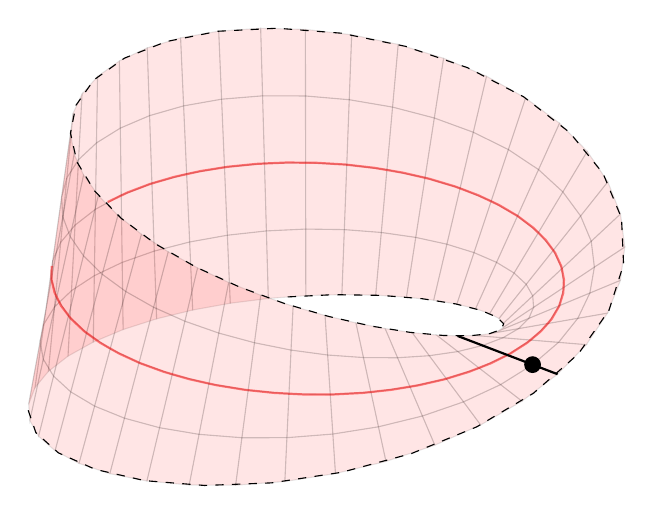
\begin{tikzpicture}
	\begin{axis}[
	hide axis,
	view={40}{40},
	width=\textwidth]
	
	\addplot3 [surf,
	red,
	opacity=0.1,
	faceted color=black,
	point meta=x,
	samples=40,
	samples y=5,
	z buffer=sort,
	domain=0:360,
	y domain=-0.5:0.5
	] (
	{(1+0.5*y*cos(x/2)))*cos(x)},
	{(1+0.5*y*cos(x/2)))*sin(x)},
	{0.5*y*sin(x/2)});
	
	% Center line
	\addplot3 [samples=50, domain=-145:180, samples y=0, red, thick, opacity=0.5
	] ({cos(x)},{sin(x)},{0});
	
	% Outside line
	\addplot3 [samples=50, domain=-135:495, samples y=0, black, dashed] (
	{(1+0.25*cos(x/2)))*cos(x)},
	{(1+0.25*cos(x/2)))*sin(x)},
	{0.25*sin(x/2)});
	
	% Glued line
	\addplot3 [samples=50,domain=-0.5:0.5,samples y=0, black, thick,
	] ({1+0.5*x},{0},{0});
	
	% Point
	\node[color=black,draw=black,circle,fill,inner sep=2pt] at (axis cs:1+1/8,0,0) {};
	\end{axis}
	\end{tikzpicture}
	\end{center}
\end{figure}

\begin{exercise}
	Check that $\sim$ is an equivalence relation, and that every equivalence class contains either one or two points. 
\end{exercise}

The \emph{M\"obius strip}\index{mobius strip@M\"obius strip} $M$ is the set of equivalence classes in $B$. In other words, we take the box $[0,1] \times (0,1)$ and ``glue'' its left and right edges, with a twist. If you've ever made a M\"obius strip out of paper, you can probably see that we've formalized exactly that same process. See \cref{mobius-box}, again.

We regard $M$ as a topological space using the quotient topology, as in \cref{quotient-space}. To give $X$ the structure of a manifold, we will construct an atlas consisting of two charts. But, before proceeding with the formalism, let's describe the intuition. Imagine making a cut in the M\"obius strip corresponding to a vertical cut in the box $B$ (ie, a cut perpendicular to the central red circle in \cref{mobius-box}). Once we make such a cut, we can untwist the M\"obius strip and we're left with an open rectangle, which we can regard as an open subset of $\R^2$. In other words, we've defined a chart on $M$. The points along the cut are missing from this chart; but if we construct a second chart by making a second separate cut, we will have constructed two charts that cover $M$. 

Let's formalize this now. The easiest place to cut is the line along which we glued the M\"obius strip in the first place. In other words, we let \[ U = \{ [a, b] \in M : a \in (0,1) \} \] 
and let $x : U \to \R^2$ be the function $x([a,b]) = (a, b)$.

\begin{exercise}
	Show that $U$ is an open subset of $M$, and that the function $x : U \to \R^2$ is well-defined, continuous, injective, and open. 
\end{exercise}

The second chart is a bit harder to describe mathematically, but the intuitive idea is the same. We'll cut the M\"obius strip along the line corresponding the vertical line $a = 1/2$ in $B$. Formally, let \[ V = \{ [a, b] \in M : a \neq 1/2 \} \] and let $y : V \to  \R^2$ be the function defined by 
\[ y([a,b]) = \begin{cases} (a, b) & \text{if } a < 1/2 \\ (a-1, 1-b) & \text{if } a > 1/2 \end{cases} \]

\begin{exercise}
	Show that $V$ is also an open subset of $M$, and that $y : V \to \R^2$ is well-defined, continuous, injective, and open. 
\end{exercise}

\begin{exercise}
	Show that $(U, x)$ and $(V, y)$ are compatible.
\end{exercise}

Thus $\mathscr{A} = \{(U, x), (V, y)\}$ is an atlas on the M\"obius strip $M$. Letting $\mathscr{A}_M$ denote the corresponding maximal atlas, we obtain the structure of a manifold on $M$.

\begin{exercise}
	Fix a constant $c \in [0,1)$, and let $U_c$ be the subset of $M$ where we've cut out the vertical line $a = c$. Show that $U_c$ is an open subset of $M$. Write down a formula for a well-defined function $x_c : U_c \to \R^2$ which is continuous, injective, and open; the image of $x_c$ should be an open box in $\R^2$, and you should recover the function $x$ above when $c = 0$, and the function $y$ when $c = 1/2$. Then show that $(U_c, x_c) \in \mathscr{A}_M$ for all $c \in [0,1)$. 
\end{exercise}

\subsection{More quotient examples}

Here is another example of a manifold you probably recognize (perhaps by the name ``donut'' rather than ``torus'') which can be constructed as a quotient space.

\begin{exercise}[Torus] \label{torus} \index{torus}
	Let $B$ denote the box $[0,1] \times [0,1]$ inside $\R^2$ and let $\sim$ denote the equivalence relation generated by $(a,0) \sim (a,1)$ and $(0,b) \sim (1,b)$ for all $a, b \in [0,1]$. The \emph{torus} $T$ is defined to be the corresponding quotient space. Describe an atlas on $T$. 
\end{exercise}

% TODO: Torus picture

But sometimes quotient spaces can be very difficult to visualize directly; the only way to have geometric intuition in these cases is to remember the space we started with before quotienting, and the equivalence relation we defined on it. 

\begin{exercise}[Projective line] \label{rp1} \index{projective line} \index{p1@$\bbP^1$|see {projective line}}
	Let $S^1$ denote the circle as in \cref{circle-projection-atlas}. Define an equivalence relation $\sim$ on $S^1$ which identifies antipodal points; in other words, every point on $S^1$ is declared to be equivalent to the point that is diametrically opposite it. The \emph{projective line} $\bbP^1$ is defined to be the corresponding quotient space. Describe an atlas on $\bbP^1$. 
\end{exercise}

\begin{exercise}[Projective plane] \label{rp2} \index{projective plane} \index{p2@$\bbP^2$|see {projective plane}}
	Let $S^2$ denote the 2-sphere as in \cref{sphere-projection-atlas}. Define an equivalence relation $\sim$ on $S^2$ which identifies antipodal points; in other words, every point on $S^2$ is declared to be equivalent to the point that is diametrically opposite it. The \emph{projective plane} $\bbP^2$ is defined to be the corresponding quotient space. Describe an atlas on $\bbP^2$. 
\end{exercise}

\subsection{Submanifolds}

\begin{definition} \label{submanifold}
	Suppose $S$ is a subset of a manifold $X$. Then $S$ is a \emph{submanifold} of $X$ if there exist charts $(U, x) \in \mathscr{A}_X$ covering $S$ such that 
	\[ S \cap U = \{ p \in U :  x_1(p) = x_2(p) = \dotsb = x_k(p) = 0 \} \]
	for some non-negative integer $k \leq \dim(U,x)$. Such a chart $(U,x)$ is said to be \emph{adapted} to $S$, and the integer $k$ is called the \emph{codimension of $S$ in $(U,x)$}. 
\end{definition}

We'll justify this terminology in a moment by showing that submanifolds are actually manifolds in their own right (cf. \cref{submanifolds-are-manifolds}). But first, let's discuss some examples. 

\begin{example}
	Consider the set $S = \{ (0,y) \in \R^2 : -1 < x < 1 \}$ inside $\R^2$. In other words, $S$ is the open interval $(-1,1)$ along the $y$-axis inside $\R^2$. Then $S$ is a submanifold. Indeed, let $U$ be the open box $(-1,1) \times (-1,1)$ inside $\R^2$, and $x : U \to \R^2$ the inclusion map. Then $(U, x)$ is a chart on $\R^2$, and 
	\[ S \cap U = \{ p \in S : x_1(p) = 0 \} \]
	so $(U,x)$ is adapted to $S$ and $S$ has codimension 1 in $(U,x)$. 
\end{example}

\begin{exercise}
	Show that each of the following is a submanifold of $\R^2$. 
	\begin{enumerate}[(a)] 
		\item The $y$-axis. 
		\item The open interval $(-1,1)$ along the $x$-axis.
		\item The line $y = x$. 
	\end{enumerate}
\end{exercise}

We now make good on our promise of proving that submanifolds are in fact manifolds. The proof is a little long because there are a lot of details to check, but there are no real tricks or surprises. 

\begin{proposition} \label{submanifolds-are-manifolds}
	Let $S$ be a submanifold of a manifold $X$. Suppose $(U, x) \in \mathscr{A}_X$ is adapted to $S$ and $S$ has codimension $k$ in $(U, x)$. Let $x|_S : S \cap U \to \R^{n-k}$ be the function defined by 
	\[ x|_S(p) = (x_{k+1}(p), \dotsc, x_n(p)). \]
	Regarding $S$ as a topological space using the subspace topology, the pair $(S \cap U, x|_S)$ is a chart on $S$, and the set of all charts of this form is an atlas on $S$. Thus $S$ becomes a manifold if we equip it with the corresponding maximal atlas $\mathscr{A}_S$. Finally, if $(U, x) \in \mathscr{A}_X$ is a chart adapted to $S$ such that $S$ has codimension $k$ in $S$, then
	\[ \dim_p(S) = \dim_p(X) - k \]
	for all $p \in S \cap U$. 
\end{proposition}

\begin{proof}
	Observe that, by definition, $x|_S$ is the composite
	\[ \begin{tikzcd}
	S \cap U \ar[hookrightarrow]{r} & U \ar{r}{x} & \R^n \ar{r}{\pi} & \R^{n-k}
	\end{tikzcd} \]
	where the first map is the inclusion, and the final map $\pi : \R^n \to \R^{n-k}$ projects onto the final $n-k$ coordinates (ie, $\pi(x_1, \dotsc, x_n) = (x_{k+1}, \dotsc, x_n)$). Each of these maps is continuous, so the composite $x|_S$ is continuous as well. The proof that $x|_S$ is injective is left as an exercise (cf. \cref{submanifolds-are-manifolds-details}). 
	
	Let us show that $x|_S$ is open. By definition of the subspace topology \ref{subspace-topology}, every open subset of $S \cap U$ is of the form $S \cap V$ where $V$ is an open subset of $U$. Suppose $p \in  S \cap V$. We want to show that $x|_S(p)$ is an interior point of $x|_S(S \cap V)$. Since $V$ is open in $U$ and $x : U \to \R^n$ is an open map, we know that $x(p)$ is an interior point of $x(V)$, ie, there exists $\epsilon > 0$ such that every point of $\R^n$ within $\epsilon$ of $x(p)$ is inside $x(V)$. We claim that the $\epsilon$ ball around $x|_S(p)$ is contained in $x|_S(S \cap V)$. Suppose we have $a = (a_{k+1}, \dotsc, a_n) \in \R^{n-k}$ such that $|a - x|_S(p)| < \epsilon$. We will show that $a \in x|_S(S \cap V)$. 
	
	Notice that, since $(U,x)$ is adapted to $S$, the vector $x(p) \in \R^n$ is the same as $x|_S(p) \in \R^{n-k}$ except that it is prepended with $k$ zeroes. Let $\iota : \R^{n-k} \to \R^n$ be the map that preprends vectors in $\R^{n-k}$ with a string of $k$ zeroes. In other words, 
	\[ \iota(b_{k+1}, \dotsc, b_n) = (\overbrace{0, \dotsc, 0}^{k \text{ times}}, b_{k+1}, \dotsc, b_n). \]
	Thus $x(p) = \iota(x|_S(p))$. Now by the definition of the euclidean norm, we see that $|\iota(a) - x(p)| = |a - x|_S(p)|$, which means that $|\iota(a) - x(p)| < \epsilon$. This means that $\iota(a) \in x(V)$ due to our choice of $\epsilon$. Since $x$ is injective, there exists a unique $q \in V$ such that $x(q) = \iota(a)$. This means that the first $k$ coordinates of $q$ are zero, so $q \in S \cap U$ since $(U, x)$ is adapted to $S$. Moreover
	\[ x|_S(q) = \pi(x(q)) = \pi(\iota(a)) = a \]
	which shows that $a \in x|_S(S \cap V)$. 
	
	Next up, suppose $(U, x)$ and $(U', x')$ are both charts in $\mathscr{A}_X$ that are adapted to $S$. We want to show that $(S \cap U, x|_S)$ and $(S \cap U', x'|_S)$ are compatible. If $S \cap U \cap U'$ is empty, there is nothing to do, so we assume that $S \cap U \cap U'$ is nonempty. Let $k$ and $k'$ be the codimensions of $S$ in the two charts $(U, x)$ and $(U', x')$, respectively. Once we prove compatibility, it follows from \cref{dimension-well-defined} that we must have $k = k'$. 
	
	The proof of compatibility is encapsulated by the following diagram. 
	\[ \begin{tikzcd}
	x|_S(S \cap U \cap U') \ar{r}{(x|_S)^{-1}} \ar{d}[swap]{\iota} & S \cap U \cap U' \ar[hookrightarrow]{d} \ar{r}{x'|_S} & x'|_S(S \cap U \cap U') \\
	x(U \cap U') \ar{r}{x^{-1}} & U \cap U' \ar{r}{x'} & x'(U \cap U') \ar{u}[swap]{\pi'}
	\end{tikzcd} \]
	Here $\iota$ denotes the ``prepend with $k$ zeroes'' map, and $\pi'$ is the ``project onto the final $k'$ coordinates'' map. You should stare at the above diagram until you've convinced yourself that it ``commutes,'' ie, that the result of following any two paths of arrows that start and end at the same place ends up being the same. (The fact that the square on the left of the diagram commutes is because $(U, x)$ is adapted to $S$, and the fact that square on the right commutes is by definition of the function $x'|_S$.)
	
	In other words, the diagram tells us that the transition function $x'|_S \circ (x|_S)^{-1}$ is equal to $\pi' \circ (x' \circ x^{-1}) \circ \iota$. Since $(U,x)$ and $(U', x')$ are compatible, we know that $x' \circ x^{-1}$ is smooth. Thus the transition function $x'|_S \circ (x|_S)^{-1}$ is smooth. 
	
	Since $S$ is a submanifold, we know that it can be covered by charts in $X$ that are adapted to $S$. Thus we've just shown that the set
	\[ \mathscr{A} = \{ (S \cap U, x|_S) : (U, x) \in \mathscr{A}_X \text{ is adapted to } S \} \]
	is an atlas on $S$. The assertion about $\dim_p(S)$ follows immediately. 
\end{proof}

\begin{exercise} \label{submanifolds-are-manifolds-details}
	Show that $x|_S$ is injective. 
\end{exercise}

We've used the word ``submanifold'' once before, in \cref{open-submanifold} where we defined ``open submanifolds.'' Let us now show that this earlier usage of the word ``submanifold'' was justified and does not produce any conflicts with our new definitions.  

\begin{exercise} \label{open-submanifolds-are-submanifolds}
	Suppose $X$ is a manifold and $U$ is an open subset. 
	\begin{enumerate}[(a)]
		\item Show that $U$ is a submanifold (in the sense of \cref{submanifold}). 
		\item Show that the maximal atlas on $U$ constructed by \cref{submanifolds-are-manifolds} is equal to the atlas described in \cref{open-submanifold}. 
	\end{enumerate}
	\begin{hint}
		Show that a chart $(V, x) \in \mathscr{A}_X$ is adapted to $U$ if and only if $V \subseteq U$, and that $U$ has codimension 0 in any such chart. 
	\end{hint}
\end{exercise}

Here is another property you would hope would be true. 

\begin{exercise}[``Submanifolds of submanifolds are submanifolds'']
	Let $X$ be a manifold, $S$ a submanifold of $X$, and $T$ a submanifold of $S$. Show that $T$ is a submanifold of $X$. 
\end{exercise}

\subsection{Submanifolds of euclidean space}

We now have two important results which let us produce lots of examples of submanifolds of euclidean space out of smooth functions (in the sense of \cref{smooth-multi}). 

First up, we have the following important theorem which goes by many names; we will call it the ``regular level set theorem,'' but some other names include the ``preimage theorem'' or the ``submersion theorem.'' We will later generalize this theorem. 

\begin{theorem}[Regular level set theorem] \label{regular-level-set-theorem-local}
	Suppose $U$ is an open subset of $\R^m$ and $f : U \to \R^n$ is a smooth function where $m \geq n$. If $q \in \R^n$ is a regular value of $f$, then $S = f^{-1}(q)$ is a submanifold of $U$ of dimension $m-n$. 
\end{theorem}

\begin{proof}
	By replacing $f$ with the function $x \mapsto f(x)-q$, we can assume without loss of generality that $q = 0$. Fix $p \in S$. We want to find a chart adapted to $S$ containing $p$. Since $0$ is a regular value and $m \geq n$, we know that $f$ is submersive at $p$. This means that the $n \times m$ matrix $f'(p)$ has a non-vanishing $n \times n$ minor, ie, there exist $n$ distinct integers $i_1, \dotsc, i_n$ between $1$ and $m$ such that 
	\begin{equation} \label{derivative-non-vanishing-minor} 
	\det \begin{bmatrix} \partial_{i_1} f_1(p) & \dotsb & \partial_{i_n} f_1(p) \\ \vdots & \ddots & \vdots \\ \partial_{i_1} f_n(p) & \dotsb & \partial_{i_n} f_n(p) \end{bmatrix} \neq 0. 
	\end{equation}
	By permuting the coordinates, we can assume without loss of generality that $i_1 = 1, i_2 = 2, \dotsc, i_n = n$ (cf. \cref{permutation-submanifold}). Consider the function $y : U \to \R^m$ such that, if $x = (x_1, \dotsc, x_m) \in U$, then
	\[ y(x) = (f_1(x), \dotsc, f_n(x), x_{n+1}, \dotsc, x_m). \]
	Then
	\[ y'(x) = 
	\begin{bmatrix} 
	\partial_1 f_1(x) & \dotsb & \partial_n f_1(x) & \partial_{n+1} f_1(x) & \dotsb & \partial_m f_1(x) \\ 
	\vdots & \dotsb & \vdots & \vdots & \ddots & \vdots \\ 
	\partial_1 f_n(x) & \dotsb & \partial_n f_n(x) & \partial_{n+1} f_n(x) & \dotsb & \partial_m f_n(x) \\
	0 & \dotsb & 0 & 1 & \dotsb & 0 \\ 
	\vdots & \ddots & \vdots & \vdots & \ddots & \vdots \\ 
	0 & \dotsb & 0 & 0 & \dotsb & 1
	\end{bmatrix} \]
	In other words, the $(m-n) \times m$ submatrix on the bottom left of $g'(x)$ is all zeroes, and the $(m-n) \times (m-n)$ submatrix on the bottom right is the identity matrix. This means that $\det y'(x)$ is equal, up to sign, to the determinant of the $n \times n$ in the top left, which we know from \cref{derivative-non-vanishing-minor} is nonzero when $x = p$. Thus $y$ is \'etale at $p$. 
	
	Since $f$ is smooth, so is $y$, so there exists an open neighborhood $V$ of $p$ such that $y|_V$ is \'etale. By the inverse function theorem \ref{inverse-function-theorem}, we can replace $V$ with a smaller open neighborhood of $p$ in order to further assume that $y|_V$ is injective. Then \cref{euclidean-chart-characterization} tells us that $(V, y)$ is a chart in the euclidean atlas containing $p$. Moreover, 
	\[ S \cap V = \{ p' \in V : f(p') = 0 \} = \{ p' \in V : y_1(p') = \dotsb = y_n(p') = 0 \} \]
	because $y_j = f_j$ for all $j = 1, \dotsc, n$. This shows that $(V,y)$ is adapted to $S$, and that $S$ has codimension $n$ at $p$ in $\R^m$. 
\end{proof}

\begin{exercise} \label{permutation-submanifold}
	Suppose $\sigma$ is a permutation of the set $\{1, \dotsc, m\}$. Let $f_\sigma : \R^m \to \R^m$ be the function which ``permutes the coordinates of elements of $\R^m$ according to $\sigma$,'' ie, 
	\[ f_\sigma(x_1, \dotsc, x_m) = (x_{\sigma(1)}, \dotsc, x_{\sigma(m)}). \]
	Show that a subset $S$ is a submanifold of $\R^m$ if and only if $f_\sigma(S)$ is a submanifold of $\R^m$. 
\end{exercise}

\begin{exercise}
	Recall from \cref{circle-projection-atlas,sphere-projection-atlas} that the $n$-sphere $S^n$ is defined by
	\[ S^n = \{ x \in \R^{n+1} : |x| = 1 \}. \]
	\begin{enumerate}[(a)]
		\item Use the regular level set theorem \ref{regular-level-set-theorem-local} to show that $S^1$ is a submanifold of $\R^{2}$. 
		\item Show that the maximal atlas on $S^1$ produced by \cref{submanifolds-are-manifolds} coincides with the maximal atlas from \cref{circle-projection-atlas}. 
		\item Generalize parts (a) and (b) to $S^n$ for arbitrary $n$. 
	\end{enumerate}
\end{exercise}

\begin{proposition} \label{graphs-smooth}
	Suppose $U$ is an open subset of $\R^m$ and $f : U \to \R^n$ is a smooth function. Then the graph of $f$ is a submanifold of $\R^{m+n}$. 
\end{proposition}

\begin{proof}
	We derive this from the regular level set theorem \ref{regular-level-set-theorem-local}. Consider the function $g : U \times \R^n \to \R^n$ given by $g(x, y) = f(x) - y$. Then the graph of $f$ is equal to $g^{-1}(0)$, so the result will follow from \cref{regular-level-set-theorem-local} provided we can show that 0 is a regular value of $g$. 
	
	In fact, $g$ is submersive at all points, so all of its values are regular! To see this, we calculate $dg$. Note that if $x = (x_1, \dotsc, x_m) \in U$ and $y = (y_1, \dotsc, y_n) \in \R^n$, then
	\[ g(x,y) = g(x_1, \dotsc, x_m, y_1, \dotsc, y_n) = (f_1(x_1,\dotsc, x_m)-y_1, \dotsc, f_n(x_1, \dotsc, x_m) - y_n) \]
	by definition of $g$, which means that
	\[ \frac{\partial g_k}{\partial x_i}(x,y) = \frac{\partial f_k}{\partial x_j}(x) = \partial_j f_k(x) \quad \text{and} \quad \frac{\partial g_k}{\partial y_j}(x,y) = -\delta_{j,k} = \begin{cases} -1 & \text{if } j = k \\ 0 & \text{if } j \neq k \end{cases} \]
	where $i = 1, \dotsc, m$ and $j, k = 1, \dotsc n$. In other words, $g'(x,y)$ is the following $n \times (m+n)$ matrix. 
	\[ g'(x,y) = 
	\begin{bmatrix} 
	\partial_1 f_1(x) & \partial_2 f_1(x) & \dotsb & \partial_m f_1(x) & -1 & 0 & \dotsb & 0 \\ 
	\partial_1 f_2(x) & \partial_2 f_2(x) & \dotsb & \partial_m f_2(x) & 0 & -1 & \dotsb & 0 \\
	\vdots & \vdots & \ddots & \vdots & \vdots & \vdots & \ddots & \vdots \\ 
	\partial_1 f_n(x) & \partial_2 f_n(x) & \dotsb & \partial_m f_n(x) & 0 & 0 & \dotsb & -1 \end{bmatrix} = \begin{bmatrix} f'(x) & -I \end{bmatrix} \]
	where $I$ denotes the $n \times n$ identity matrix. Since $I$ has rank $n$, so does $g'(x,y)$, proving that $g$ is submersive everywhere. 
\end{proof}

An important cautionary remark is that sometimes, a subspace that is a manifold can fail to be a submanifold. For example, you might notice that we showed in \cref{graphs-continuous} that the graph of a \emph{continuous} function between two euclidean spaces is a subspace of euclidean space and is also a manifold; and then we showed in \cref{graphs-smooth} that the graph of a \emph{smooth} function is a submanifold of euclidean space. And indeed, the graphs of continuous-but-not-smooth functions provide examples of subspaces that are manifolds but not submanifolds. 

\begin{exercise}
	Let $f : \R \to \R$ be the function $f(x) = |x|$. Show that the graph of $f$ is not a submanifold of $\R^2$. 
\end{exercise}

\section{Smooth functions}

We will now define what it means for a function between two manifolds to be smooth. Recall that in \cref{multi} we saw that the case when the codomain is $\R$ was the most important. The same will be true here. You may find that the number of definitions of ``smooth'' gets slightly out of hand; if you do, just remember that, whenever multiple definitions of ``smooth'' make sense, they'll all agree. 

\subsection{Smooth real-valued functions}

\subsubsection*{Definition of smoothness for real-valued functions}

\begin{definition}[Smooth real-valued function] \label{smooth-real-valued} \index{smooth}
	Let $X$ be a manifold. A function $f : X \to \R$ is said to be \emph{smooth} if, for any chart $(U, x) \in \mathscr{A}_X$, the function $f \circ x^{-1}$ is smooth.
	\[ \begin{tikzcd} x(U) \ar{r}{x^{-1}} & U \ar{r}{f} & \R \end{tikzcd} \]
\end{definition}

There are two disconcerting things about this definition. First, there is the issue that checking smoothness of a particular function seems next to impossible: the maximal atlas $\mathscr{A}_X$ will have \emph{many, many} charts, some that we may not even know about, and the definition makes it seem like we need to check smoothness on all of them! Thankfully, we don't need to check on all possible charts. As soon as we check smoothness on any atlas, even if it's not maximal, we're done. 

\begin{lemma} \label{smooth-real-valued-local}
	Let $X$ be a manifold and $f : X \to \R$ a function. Suppose that there exists an atlas $\mathscr{A} \subseteq \mathscr{A}_X$ such that $f \circ x^{-1}$ is smooth for any $(U, x) \in \mathscr{A}$. Then $f$ is smooth. 
\end{lemma}

\begin{proof}
	Suppose $(V, y) \in \mathscr{A}_X$. For any $(U, x) \in \mathscr{A}$, we have maps as follows.
	\[ \begin{tikzcd} y(U \cap V) \ar{r}{y^{-1}} \ar{d}[swap]{x \circ y^{-1}} & U \cap V \ar{r}{f} & \R \\ x(U \cap V) \ar[bend right]{ur}[swap]{x^{-1}} \end{tikzcd} \]
	Since $(V, y)$ and $(U, x)$ are both elements of the maximal atlas $\mathscr{A}_X$, we know that the transition function $x \circ y^{-1}$ is smooth. Since $(U, x) \in \mathscr{A}$, we know by assumption that $f \circ x^{-1}$ is smooth. Thus \[ f \circ y^{-1} = (f \circ x^{-1}) \circ (x \circ y^{-1}) \]
	is a smooth function $y(U \cap V) \to \R$. 
	
	Now note that, since $\mathscr{A}$ is an atlas, its charts cover all of $X$, so
	\[ \bigcup_{(U,x) \in \mathscr{A}} y(U \cap V) = y(V). \]
	Since $f \circ y^{-1}$ is smooth when restricted to each the open subset $y(U \cap V)$ for all $(U, x) \in \mathscr{A}$, we conclude that $f \circ y^{-1}$ must be smooth on all of $y(V)$.
\end{proof}

The second disconcerting thing is the following. Suppose $U \subseteq \R^m$ is an open subset and $f : U \to \R$ is a function. On the one hand, we defined what it means for $f$ to be smooth back in \cref{smooth-multi}. On the other hand, we can regard $U$ as an open submanifold of $\R^n$ (cf. \cref{open-submanifold}) and then \cref{smooth-real-valued} gives us another definition of what it means for $f$ to be smooth. A priori, it could be that these definitions conflict. Thankfully, they do not. 

\begin{exercise}
	Suppose $U \subseteq \R^m$ is an open subset and $f : U \to \R$ is a function. Show that $f$ is smooth in the sense of \cref{smooth-multi} if and only if it is smooth in the sense of \cref{smooth-real-valued}. 
	\begin{hint}
		You might find \cref{smooth-real-valued-local} useful. 
	\end{hint}
\end{exercise}

From here on out, we'll use the fact that these two definitions of smoothness coincide without comment. 

\subsubsection*{Combining smooth real-valued functions}

\begin{definition}
	If $X$ is a manifold, we write $\O(X)$ for the set of smooth functions $X \to \R$. 
\end{definition}

Here is the standard set of stability properties we would want. 

\begin{exercise} \label{smooth-real-valued-stable}
	\begin{enumerate}[(a)]
		\item Show that $\O(X)$ is a vector space. 
		\item If $f, g \in \O(X)$, show that $fg \in \O(X)$ also. 
		\item If $f \in \O(X)$ and $f(x) \neq 0$ for all $x$, show that $1/f \in \O(X)$ also. 
		\begin{hint}
			You might decide to do part (d) first, and then use it to prove (c). Or not, you could also just prove (c) directly. 
		\end{hint}
		\item Suppose $f \in \O(X)$, $U$ is an open subset of $\R$, $g : U \to \R$ is smooth, and $f(X) \subseteq U$. Show that $g \circ f \in \O(X)$. 
	\end{enumerate}
\end{exercise}

\begin{unimportantremark}
	if you've taken abstract algebra, you might be interested to notice that the first two stability properties in \cref{smooth-real-valued-stable} show that $\O(X)$ is an $\R$-algebra (ie, that it is simultaneously a commutative ring and a vector space, and that these two structures are ``compatible'' with each other). 
\end{unimportantremark}

\subsubsection*{Smooth approximations of characteristic functions of compact subsets \starred}

Here is a generalization of \cref{constant-compact-zero-outside-neighborhood} which proves, roughly speaking, that we can find a smooth approximation of the characteristic function of a compact subset of a manifold. You may want to look at \cref{compact-topological-space} for the definition of compactness for topological spaces. 

\begin{proposition} \label{smooth-approximation-characteristic-compact}
	Suppose $K$ is a compact subset of a manifold $X$ and $U$ is an open neighborhood of $K$. Then there exists a smooth function $f \in \O(X)$ such that $0 \leq f(x) \leq 1$ for all $x \in \R$, $f(x) = 1$ for all $x \in K$, and $f(x) = 0$ for all $x \notin U$. 
\end{proposition}

\begin{proof}
	Suppose $(V, x)$ is a chart containing some $p \in K$. Recentering, we can assume that $x(p) = 0$ (cf. \cref{recentering-chart}). By shrinking $V$, we can assume that $\bar{V} \subseteq U$ (cf. \cref{smooth-approximation-characteristic-compact-details}). Then $x(V)$ is an open neighborhood of $0 = x(p) \in \R^n$, so there exists $\epsilon > 0$ such that $B(0, \epsilon) \subseteq x(V)$. Let $\psi : \R^n \to \R$ be a bump function supported on $\overline{B}(0, \epsilon)$ (cf. \cref{multivariable-bump-round-support}). Then $\psi \circ x$ is a smooth function on $V$ (cf. \cref{smooth-approximation-characteristic-compact-details}) which is supported entirely inside $V$ (namely, on $x^{-1}(\overline{B}(0,\epsilon))$), and is zero everywhere else on $V$. Define $f_p : X \to \R$ by
	\[ f_p(x) = \begin{cases} \psi \circ x & \text{if } x \in V \\ 0 &  \text{if } x \notin V. \end{cases} \]
	Then $f_p$ is smooth (cf. \cref{smooth-approximation-characteristic-compact-details}), and it is strictly positive on an open neighborhood $V_p$ of $p$ contained inside $U$.  
	
	We can construct such a function $f_p$ for every $p \in K$. Since $K$ is compact, there exist finitely many $p_1, \dotsc, p_n \in K$ such that $K \subseteq V_{p_1} \cup \dotsb \cup V_{p_n}$. Thus $f_{p_1} + \dotsb + f_{p_n}$ is strictly positive on $K$, and zero outside $U$. Since $K$ is compact, there exists $\delta > 0$ such that $f_{p_1} + \dotsb + f_{p_n} \geq \delta$ on $K$ (cf. \cref{smooth-approximation-characteristic-compact-details}). Let $g$ be a bridging function such that $g(x) = 1$ for $x \geq \delta$ and $g(x) = 0$ for $x \leq 0$ (cf. \cref{bridge-function}), and then set $f = g \circ (f_{p_1} + \dotsb + f_{p_n})$.
\end{proof}

\begin{exercise} \label{smooth-approximation-characteristic-compact-details}
	Fill in the missing details in the above proof. 
	\begin{enumerate}[(a)]
		\item Prove that we can ``shrink $V$ in order to assume that $\bar{V} \subseteq U$.''
		\item Modify the bump function of \cref{multivariable-bump-round-support} so that it has support $\overline{B}(0, \epsilon)$. 
		\item Explain why $\psi \circ x$ is a smooth function $V \to \R$. 
		\item Explain why $f_p$ is a smooth function $X \to \R$. 
		\item If $h : K \to \R$ is a continuous function such that $h(x) > 0$ for all $x \in K$, show that there exists $\delta > 0$ such that $h(x) \geq \delta$ for all $x$. 
		
		\begin{hint}
			Let $\delta = \inf\{ h(x) : x \in K \}$ and recall the extreme value theorem. 
		\end{hint}
	\end{enumerate}
\end{exercise}

% TODO: Partitions of unity

\subsection{Smooth functions between manifolds}

Here is a definition that may look a bit terrifying at first. 

\begin{definition}[Smoothness] \label{smooth-between-manifolds} \index{smooth}
	Suppose $X$ and $Y$ are manifolds and $f : X \to Y$ is a function. Then $f$ is \emph{smooth} if, for every chart $(V, y) \in \mathscr{A}_Y$ and every chart $(U, x) \in \mathscr{A}_X$ such that $f(U) \subseteq V$, the function $y \circ f \circ x^{-1} : x(U) \to y(V)$ is smooth. 
	\[ \begin{tikzcd} X \ar{rr}{f} && Y \\ 
	U \ar{rr}{f} \ar[hookrightarrow]{u} \ar{d}[swap]{x} &&  V \ar[hookrightarrow]{u} \ar{d}{y} \\ 
	x(U) \ar{rr}{y \circ f \circ x^{-1}} \ar[hookrightarrow]{d} && y(V) \ar[hookrightarrow]{d} \\ 
	\R^m && \R^n \end{tikzcd} \]
\end{definition}

Once again, we don't need to check all possible charts. The statement is a bit complicated, but it's exactly the statement you might hope for.  

\begin{exercise} \label{smooth-local}
	Suppose $X$ and $Y$ are manifolds and $f : X \to Y$ is a function. Suppose further that there exists an atlas $\mathscr{A} \subseteq \mathscr{A}_Y$ such that, for every $(V, y) \in \mathscr{A}$, there exists an atlas $\mathscr{A}' \subseteq \mathscr{A}_{f^{-1}(V)}$, such that for every $(U, x) \in \mathscr{A}'$, the function $y \circ f \circ x^{-1} : x(U) \to y(V)$ is smooth. Show that $f$ is smooth.
\end{exercise}

We should also note that we haven't redefined the word ``smooth'' in any conflicting ways. More precisely, we have the following two exercises. 

\begin{exercise}
	If $U \subseteq \R^m$ is an open subset and $f : U \to \R^n$ is a function, show that $f$ is smooth in the sense of \cref{smooth-multi} if and only if it is smooth in the sense of \cref{smooth-between-manifolds}.
\end{exercise}

\begin{exercise}
	Show that a function $f : X \to \R$ is smooth in the sense of \cref{smooth-real-valued} if and only if it is smooth in the sense of \cref{smooth-between-manifolds}.
\end{exercise}

From here on out, we'll use the fact that all of these definitions of smoothness coincide without comment. 

Here is an important example of a smooth function. 

\begin{exercise} \label{universal-cover-circle}
	Let $f : \R \to S^1$ be the function $f(t) = (\cos(t), \sin(t))$. Show that $f$ is smooth. 
\end{exercise}

% TODO: Pictures of the universal cover of the circle

\subsubsection*{Combining smooth maps}

It doesn't make sense to add or multiply maps that take values in a manifold. The only thing that makes sense is composition, and indeed, we can compose. 

\begin{exercise} \label{smooth-stable-composite}
	Suppose $X, Y, Z$ are all manifolds and $f : X \to Y$ and $g : Y \to Z$ are smooth. Show that $g \circ f$ is also smooth. 
\end{exercise}  

\subsubsection*{Reduction to smooth real-valued functions}

Finally, we show that the case when the codomain is $\R$ is the most important case. We do this in two steps. 

\begin{proposition} \label{euclidean-valued-smooth-iff-components-smooth}
	Suppose $X$ is a manifold and $f : X \to \R^n$ is a function. Then $f$ is smooth if and only if the component functions $f_i = \pi_i \circ f$ are smooth for all $i = 1, \dotsc, n$. 
\end{proposition}

\begin{proof}
	The single chart $(\R^n, \id)$ is a sub-atlas of the euclidean atlas on $\R^n$, so \cref{smooth-local} says that $f$ is smooth if and only if, for every $(U, x) \in \mathscr{A}_X$, the composite $f \circ x^{-1} : x(U) \to \R^n$ is smooth. This is a function from an open subset of euclidean space into euclidean space, so we know from the definition of smoothness in \cref{multi} that $f \circ x^{-1}$ is smooth if and only if its component functions $\pi_i \circ (f \circ x^{-1})$ are smooth for all $i$. But 
	\[ \pi_i \circ (f \circ x^{-1}) = (\pi_i \circ f) \circ x^{-1} = f_i \circ x^{-1}, \]
	and $f_i \circ x^{-1}$ is smooth for all $(U, x) \in \mathscr{A}_X$ if and only if $f_i$ is smooth, again by \cref{smooth-local}. 
\end{proof}

\begin{proposition} \label{smooth-iff-real-valued-pullbacks-smooth}
	Suppose $f : X \to Y$ is a function between two manifolds. Then the following are equivalent. 
	\begin{enumerate}[(a)]
		\item $f$ is smooth. 
		\item For every open subset $V \subseteq Y$ and every smooth function $g :  V \to \R$, the composite $g \circ f|_{f^{-1}(V)}$ is a smooth function $f^{-1}(V) \to \R$. 
	\end{enumerate}
\end{proposition}

\begin{proof}
	One direction follows immediately from \cref{smooth-stable-composite}. Conversely, suppose $f$ has the property described in (b). Choose a chart $(V, y) \in \mathscr{A}_Y$ of dimension $n$. By assumption, $y_i \circ f|_{f^{-1}(V)}$ is a smooth function $f^{-1}(V) \to \R$ for all $i = 1, \dotsc, n$. By \cref{euclidean-valued-smooth-iff-components-smooth}, this means that $y \circ f|_{f^{-1}(V)}$ is smooth. Since this is true for all charts $(V, y) \in \mathscr{A}_Y$, we conclude that $f$ is smooth.  
\end{proof}

\begin{unimportantremark}
	Suppose $f : X \to Y$ is a smooth function between manifolds. For any $g \in \O(Y)$, we have $g \circ f \in \O(X)$. Thus $g \mapsto g \circ f$ defines a function $f^\sharp : \O(Y) \to \O(X)$, which is actually a homomorphism of $\R$-algebras.
\end{unimportantremark}

\subsection{Paths}

{\color{blue} Incomplete. Gist: we can do basically all we did in \cref{paths-multi} on manifolds, too.}

% TODO: Paths

\subsection{Diffeomorphisms}

Diffeomorphisms are how we formalize the idea that two manifolds are ``basically the same.''

\begin{definition}[Diffeomorphism] \index{diffeomorphism}
	Suppose $X$ and $Y$ are manifolds. A function $f : X \to Y$ is a \emph{diffeomorphism} if it is smooth, bijective, and the inverse function $f^{-1} : Y \to X$ is also smooth. If there exists a diffeomorphism $f : X \to Y$, then $X$ and $Y$ are \emph{diffeomorphic}. 
\end{definition}

\begin{exercise}
	Regard $\R$ as a manifold in two different ways: once with the euclidean atlas, and next with the maximal atlas containing $(\R, x \mapsto x^3)$. Show that these two manifolds are diffeomorphic. 
\end{exercise}

\begin{exercise}
	If $X$ is a manifold and $(U, x) \in \mathscr{A}_X$, prove that $x : U \to x(U)$ is a diffeomorphism. 
\end{exercise}

\begin{definition}[Local diffeomorphism] \index{local diffeomorphism|see {diffeomorphism, local diffeomorphism}} \index{diffeomorphism!local diffeomorphism}
	Suppose $X$ and $Y$ are manifolds. A function $f : X \to Y$ is a \emph{local diffeomorphism} if, for every $p \in X$, there exists an open neighborhood $U$ of $p$ such that $f(U)$ is an open subset of $Y$ and $f|_U$ is a diffeomorphism $U \to f(U)$. 
\end{definition}

\begin{exercise} \label{universal-cover-circle-local-diffeomorphism}
	Consider the smooth function $f : \R \to S^1$ given by $f(t) = (\cos(t), \sin(t))$ from \cref{universal-cover-circle}. Show that $f$ is a local diffeomorphism. 
\end{exercise}

\begin{exercise}
	Show that local diffeomorphisms are smooth and open. 
\end{exercise}